\section{Introducción y alcance de esta entrega}

Este documento presenta el avance correspondiente a la \textbf{Fase 1} del proyecto
\emph{Sistema de Animación de Océano}: generación de la malla base y animación de
oleaje mediante superposición de ondas sinusoidales (modelo de Gerstner/suma de senos).
Quedan fuera del alcance de esta entrega, y se abordarán en fases posteriores, el
cálculo de normales para iluminación, el mapeo de texturas y el control interactivo
de cámara.

\section{Organización y configuración del entorno}

Para mantener el proyecto escalable, el código se organiza en una estructura de directorios separando fuentes, cabeceras y recursos:

\inputminted[
    frame=lines,
    framesep=2mm,
    baselinestretch=1.2,
    fontsize=\footnotesize,
    linenos,
    breaklines,
    tabsize=4,
    xleftmargin=20pt
]{text}{resources/cod/estructura_carpetas.txt}

Se inicializó el control de versiones con Git y se configuró un \texttt{.gitignore} para excluir binarios y artefactos de compilación.

El código fuente del proyecto y los recursos asociados se encuentran disponibles en el repositorio del grupo:

\begin{center}
    \url{https://github.com/PrincceMH/VisualizacionOcean}
\end{center}

\section{Arquitectura del sistema}

El sistema se organiza en tres clases con responsabilidades separadas:

\subsection{WPoint --- el vértice}

Unidad básica de la malla. Almacena posición, normal (reservada para la fase de
iluminación) y coordenadas UV (reservadas para la fase de texturizado).

\inputminted[
    frame=lines,
    framesep=2mm,
    baselinestretch=1.2,
    fontsize=\footnotesize,
    linenos,
    breaklines,
    tabsize=4,
    xleftmargin=20pt
]{cpp}{resources/cod/WPoint.cpp}

\subsection{Wave --- la ola}

Encapsula los parámetros físicos de una ola individual: amplitud, frecuencia,
dirección y fase. Provee el cálculo del número de onda $k$, necesario para la
fórmula de desplazamiento:

\[
k = \frac{4\pi^2 f^2}{g}, \qquad g = 9.81 \; \text{m/s}^2
\]

\inputminted[
    frame=lines,
    framesep=2mm,
    baselinestretch=1.2,
    fontsize=\footnotesize,
    linenos,
    breaklines,
    tabsize=4,
    xleftmargin=20pt
]{cpp}{resources/cod/Wave.cpp}

\subsection{Ocean --- el controlador}

Administra la malla 2D de vértices, la lista de olas cargadas desde
\texttt{data/spectrum.txt} y las operaciones de ciclo de vida (actualización,
cálculo de normales y dibujo).

\inputminted[
    frame=lines,
    framesep=2mm,
    baselinestretch=1.2,
    fontsize=\footnotesize,
    linenos,
    breaklines,
    tabsize=4,
    xleftmargin=20pt
]{cpp}{resources/cod/Ocean.cpp}

\section{Generación de la malla base}

Se implementó la lógica para construir la base del océano sobre el plano $XZ$.
La cuadrícula se centra dinámicamente respecto al origen para quedar bien
posicionada frente a la cámara; todos los vértices inician con altura $y=0$ y
normal apuntando hacia arriba, listos para ser deformados en la etapa de
animación.

\inputminted[
    frame=lines,
    framesep=2mm,
    baselinestretch=1.2,
    fontsize=\footnotesize,
    linenos,
    breaklines,
    tabsize=4,
    xleftmargin=20pt
]{cpp}{resources/cod/malla.cpp}

\section{Renderizado en modo alambre}

Para validar visualmente que la topología de la superficie es correcta antes de
introducir desplazamiento vertical, iluminación o texturas, se renderiza la malla
en modo alambre (\texttt{GL\_LINE}) usando GLUT.

\inputminted[
    frame=lines,
    framesep=2mm,
    baselinestretch=1.2,
    fontsize=\footnotesize,
    linenos,
    breaklines,
    tabsize=4,
    xleftmargin=20pt
]{cpp}{resources/cod/alambre.cpp}

 \begin{figure}[H]
 \centering
 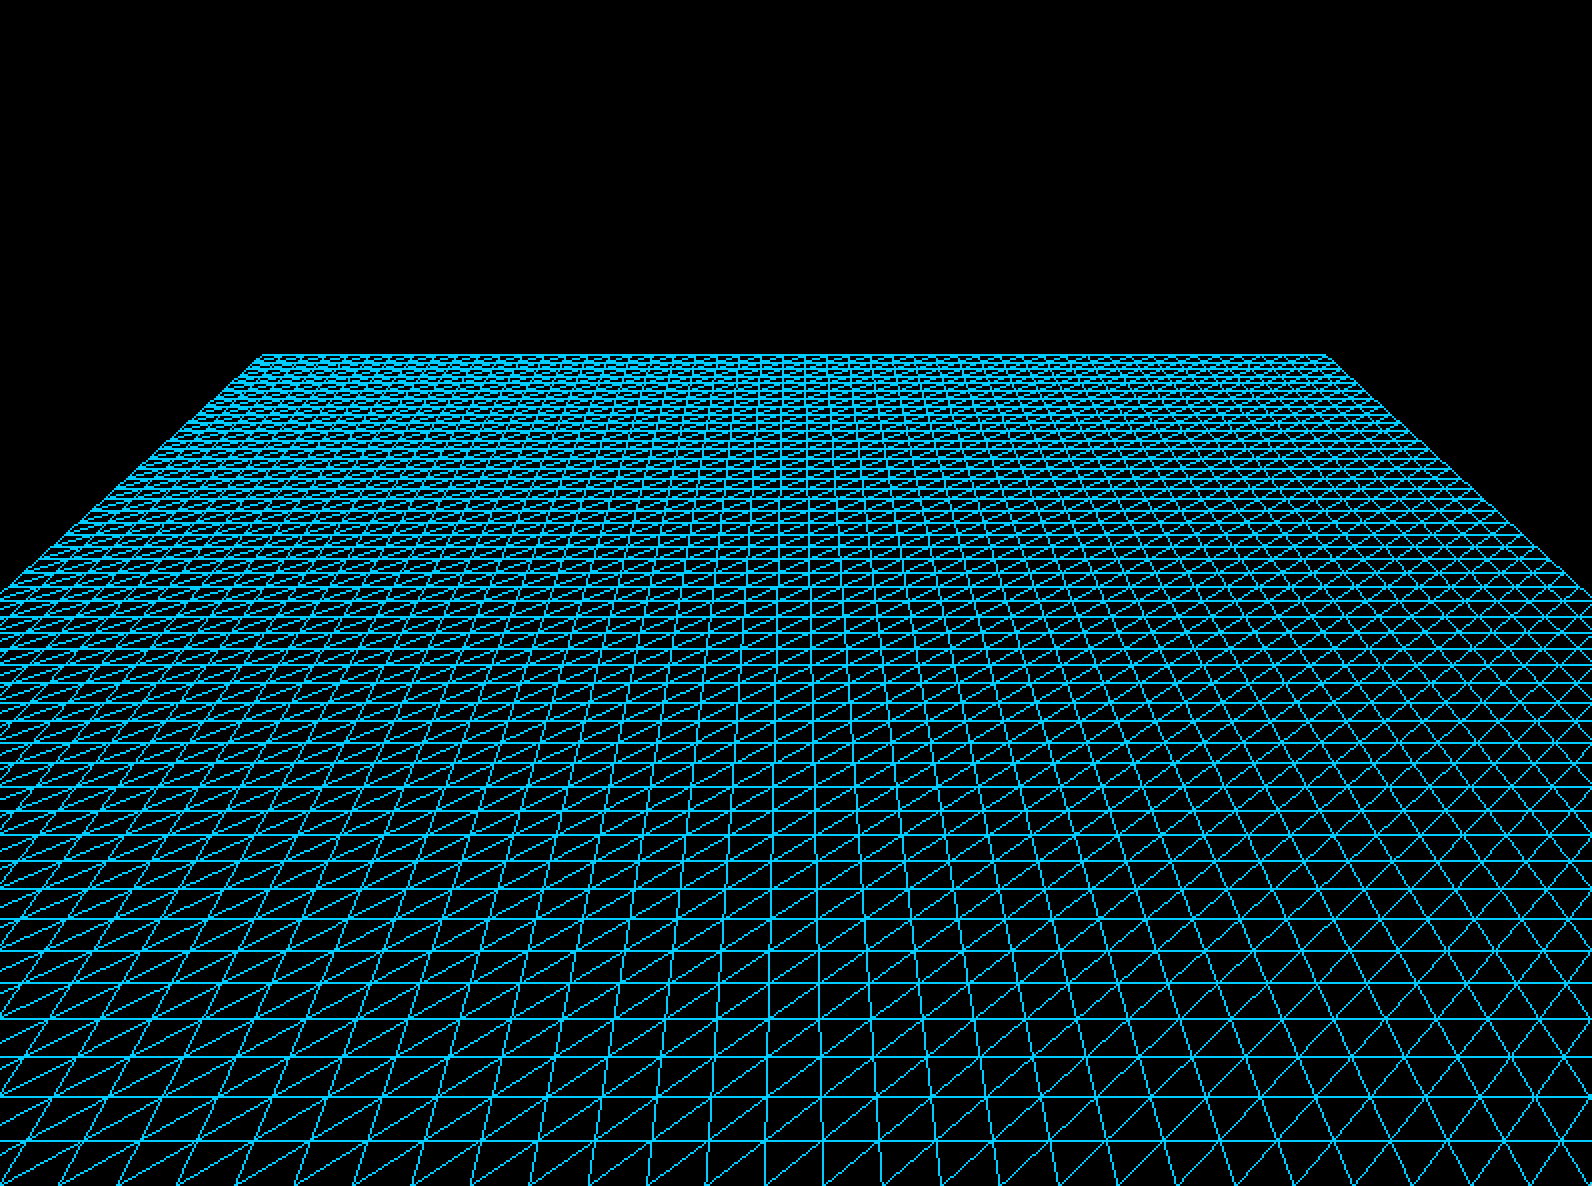
\includegraphics[width=0.8\textwidth]{figuras/malla_plana_alambre.png}
 \caption{Malla base plana renderizada en modo alambre, estado real del código en este avance.}
 \end{figure}

\section{Animación del oleaje}

Con la topología de la malla validada, se implementó la carga del espectro de
olas y la actualización temporal de la altura de cada vértice, siguiendo la
fórmula de superposición de ondas sinusoidales indicada en los requerimientos
del laboratorio:

\[
h(x, z, t) = \sum_{i=1}^{n} A_i \cos\big(k_i (x \cos(d_i) + z \sin(d_i)) - 2\pi f_i t + p_i\big)
\]

\texttt{Ocean::loadWaves()} lee de \texttt{data/spectrum.txt} la amplitud, la
dirección y la frecuencia de cada ola (una por línea) y genera una fase
aleatoria para cada una, tal como permite el enunciado:

\inputminted[
    frame=lines,
    framesep=2mm,
    baselinestretch=1.2,
    fontsize=\footnotesize,
    linenos,
    breaklines,
    tabsize=4,
    xleftmargin=20pt
]{cpp}{resources/cod/loadWaves.cpp}

\texttt{Ocean::update(float time)} recorre la malla y evalúa $h(x, z, t)$ sumando
la contribución de cada ola cargada:

\inputminted[
    frame=lines,
    framesep=2mm,
    baselinestretch=1.2,
    fontsize=\footnotesize,
    linenos,
    breaklines,
    tabsize=4,
    xleftmargin=20pt
]{cpp}{resources/cod/update.cpp}

En \texttt{main.cpp} se agregó un \texttt{glutIdleFunc} que avanza el tiempo de simulación consultando el reloj de GLUT y solicita el redibujado en cada
cuadro, logrando la animación continua del oleaje:

\inputminted[
    frame=lines,
    framesep=2mm,
    baselinestretch=1.2,
    fontsize=\footnotesize,
    linenos,
    breaklines,
    tabsize=4,
    xleftmargin=20pt
]{cpp}{resources/cod/idle.cpp}

Adicionalmente se implementó \texttt{Ocean::computeNormals()}, que calcula la
normal de cada vértice por diferencias centrales de altura respecto a sus
vecinos en $x$ y $z$. Aún no se usa para iluminación en esta fase, pero deja
la base lista para la siguiente etapa del proyecto.

\begin{figure}[H]
\centering
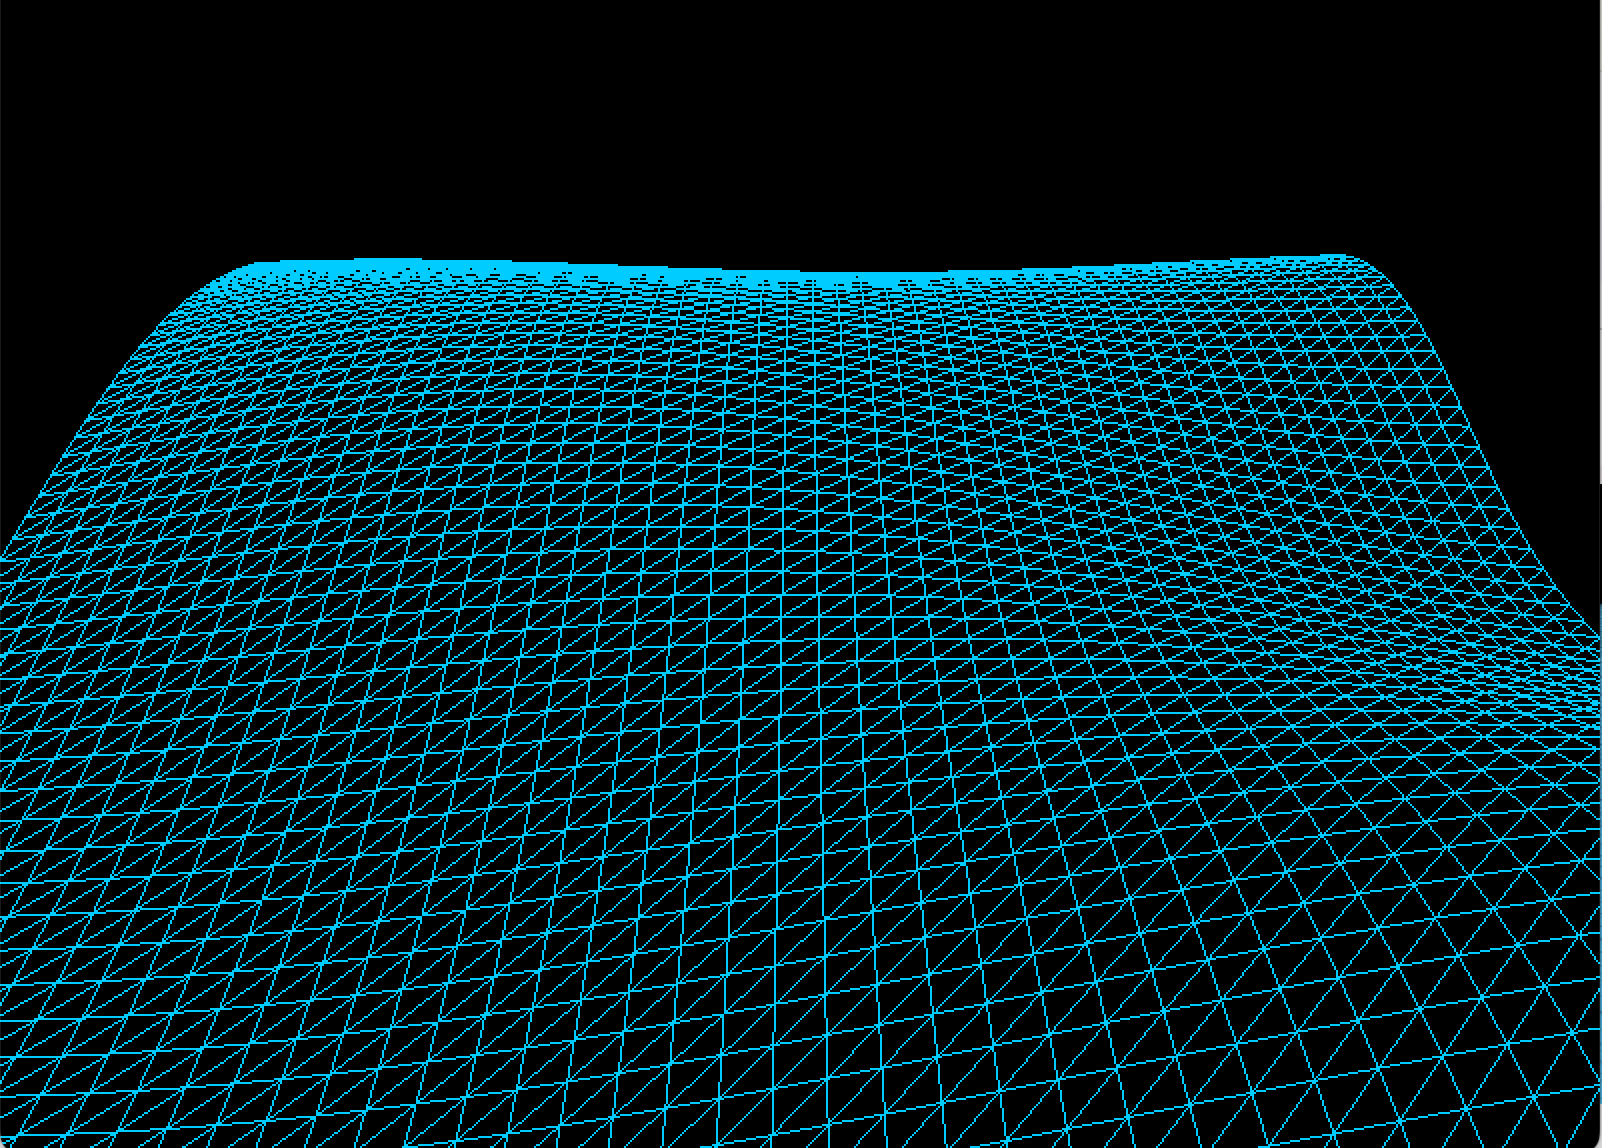
\includegraphics[width=0.8\textwidth]{figuras/oceano_animado.png}
\caption{Superficie del océano deformada por la suma de olas, renderizada en modo alambre con \texttt{update()} activo.}
\end{figure}

\section{Estado pendiente de esta fase}

Con la animación de olas funcionando, lo que queda declarado en la interfaz
pero aún no implementado corresponde a fases posteriores del proyecto:

\begin{itemize}
  \item \texttt{Ocean::loadTexture()}: carga y aplicación de la textura
        \texttt{ocean.tga} sobre la malla usando las coordenadas UV.
  \item Iluminación y materiales: activar \texttt{GL\_LIGHTING}, definir
        componentes ambiental/difusa/especular y usar las normales ya
        calculadas por \texttt{computeNormals()}.
  \item Cámara interactiva: rotación, zoom y controles de teclado para
        velocidad de animación, textura e iluminación.
  \item Elementos adicionales a la escena (mínimo dos): cielo/fondo, barco,
        isla o similar, integrados con posición, escala e iluminación propias.
\end{itemize}

\section{Conclusiones parciales}

Se cuenta con una arquitectura orientada a objetos clara, la generación de la malla base validada visualmente y, en esta entrega, la animación de oleaje funcionando de extremo a extremo: carga del espectro de olas desde archivo, cálculo de altura por superposición de senos en cada cuadro y cálculo de normales por vértice. El siguiente paso es incorporar iluminación, texturizado, cámara interactiva y los elementos adicionales de la escena.

